\section{Resultados y análisis}
% Máximo: 4 páginas
 
\subsection{Complejidad te\'orica}
Sea $L=N+M-2$ la cantidad de movimientos de un camino.
\begin{itemize}
  \item \textbf{Fuerza bruta:} enumera los $\binom{N+M-2}{N-1}$ caminos
        posibles y eval\'ua cada uno en $O(N+M)$, por lo que su tiempo es
        exponencial en el tama\~no de la grilla. Su memoria adicional es
        $O(N+M)$ (pila de recursi\'on y camino actual).
  \item \textbf{Programaci\'on din\'amica:} el estado es
        $(i,j,k)$, con $k<V$ minas detonadas, y cada estado se calcula en
        $O(1)$. Tiempo $O(NMV)$ y memoria $O(NMV)$, ya que se almacenan la
        tabla de puntajes y la de predecesores para reconstruir el camino.
  \item \textbf{Greedy:} En cada paso avanza a la celda vecina (derecha o abajo) de mayor aporte inmediato, evitando murallas y minas cuando queda una sola vida; ante empate avanza a la derecha. Toma una
        decisi\'on local en cada paso, por lo que su tiempo es $O(N+M)$ y su
        memoria $O(N+M)$ por el camino construido, sin garant\'ia de
        optimalidad ni de encontrar un camino v\'alido.
\end{itemize}
 
\subsection{Tiempo de ejecuci\'on}
La Figura~\ref{fig:tiempo} muestra el tiempo promedio en funci\'on del tama\~no
$N\cdot M$ para cada tipo de grilla, en escala log-log.
 
\begin{figure}[H]
  \centering
  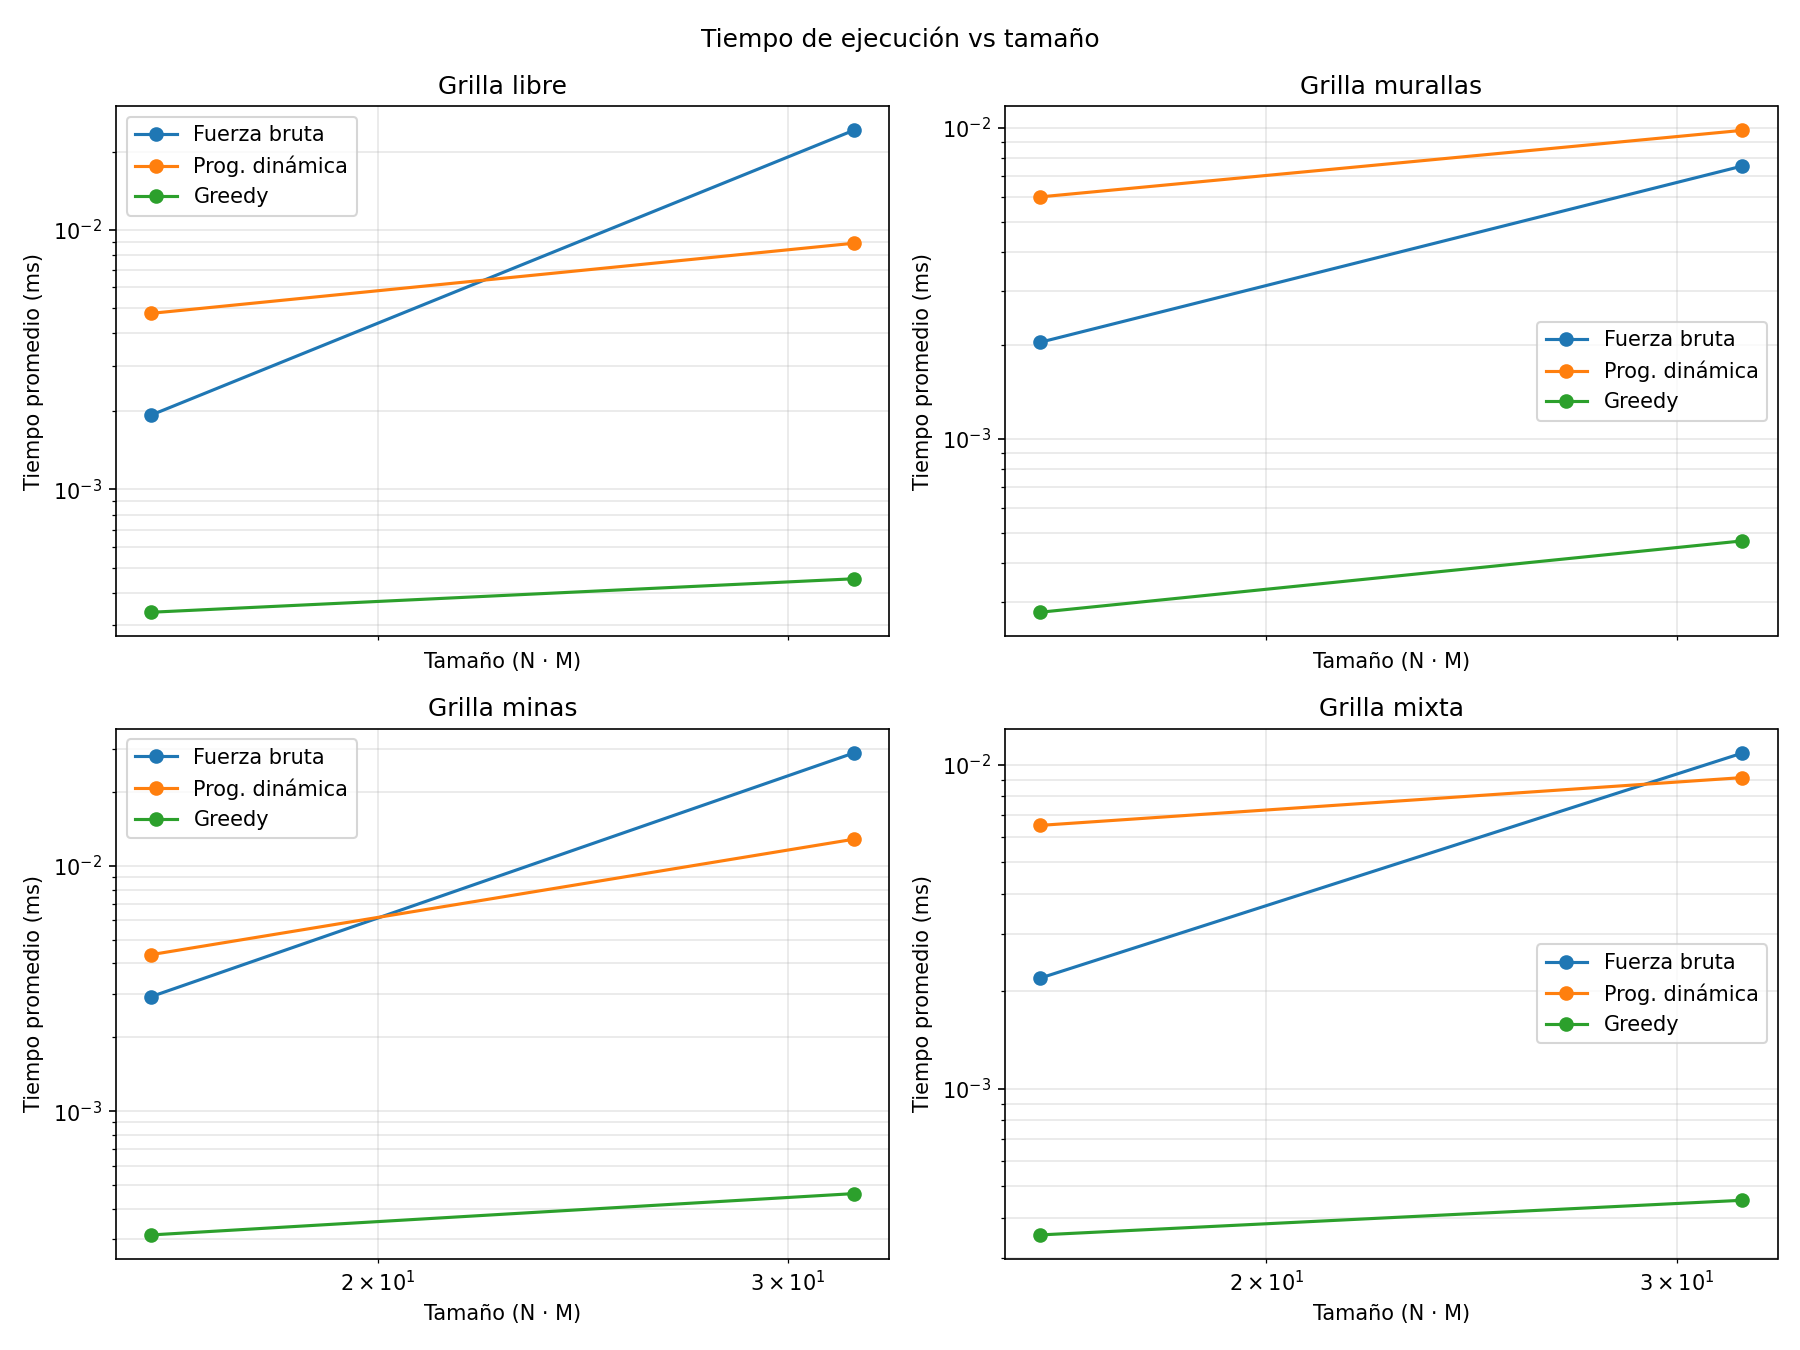
\includegraphics[width=0.95\textwidth]{plots/tiempo_vs_tamano.png}
  \caption{Tiempo de ejecuci\'on promedio vs tama\~no ($N\cdot M$), por tipo de grilla.}
  \label{fig:tiempo}
\end{figure}
 
En $4\times4$ el tiempo promedio fue de 0,010~ms para fuerza bruta, 0,043~ms
para DP y 0,0017~ms para greedy; en $4\times8$ fue de 0,054, 0,054 y
0,0020~ms, respectivamente (Tabla~\ref{tab:resumen}). Al duplicar el tama\~no,
la fuerza bruta se multiplica por 5,3, lo que concuerda en orden de magnitud con
su crecimiento exponencial: la cantidad de caminos pasa de $\binom{6}{3}=20$ a
$\binom{10}{3}=120$. DP crece solo $\times1{,}3$ y greedy $\times1{,}2$, coherente con
$O(NMV)$ y $O(N+M)$, pero con tiempos de microsegundos y una sola medici\'on
por instancia el ruido y los costos fijos (reserva de tablas) dominan, por lo
que con dos tama\~nos no se puede confirmar la pendiente log-log esperada.
Greedy es el m\'as r\'apido en todos los casos. Fuerza bruta y DP entregaron el
mismo puntaje en las 48 instancias, lo que respalda la correcci\'on de DP.
 
\subsection{Uso de memoria}
La Figura~\ref{fig:memoria} muestra la memoria adicional promedio de cada
algoritmo.
 
\begin{figure}[H]
  \centering
  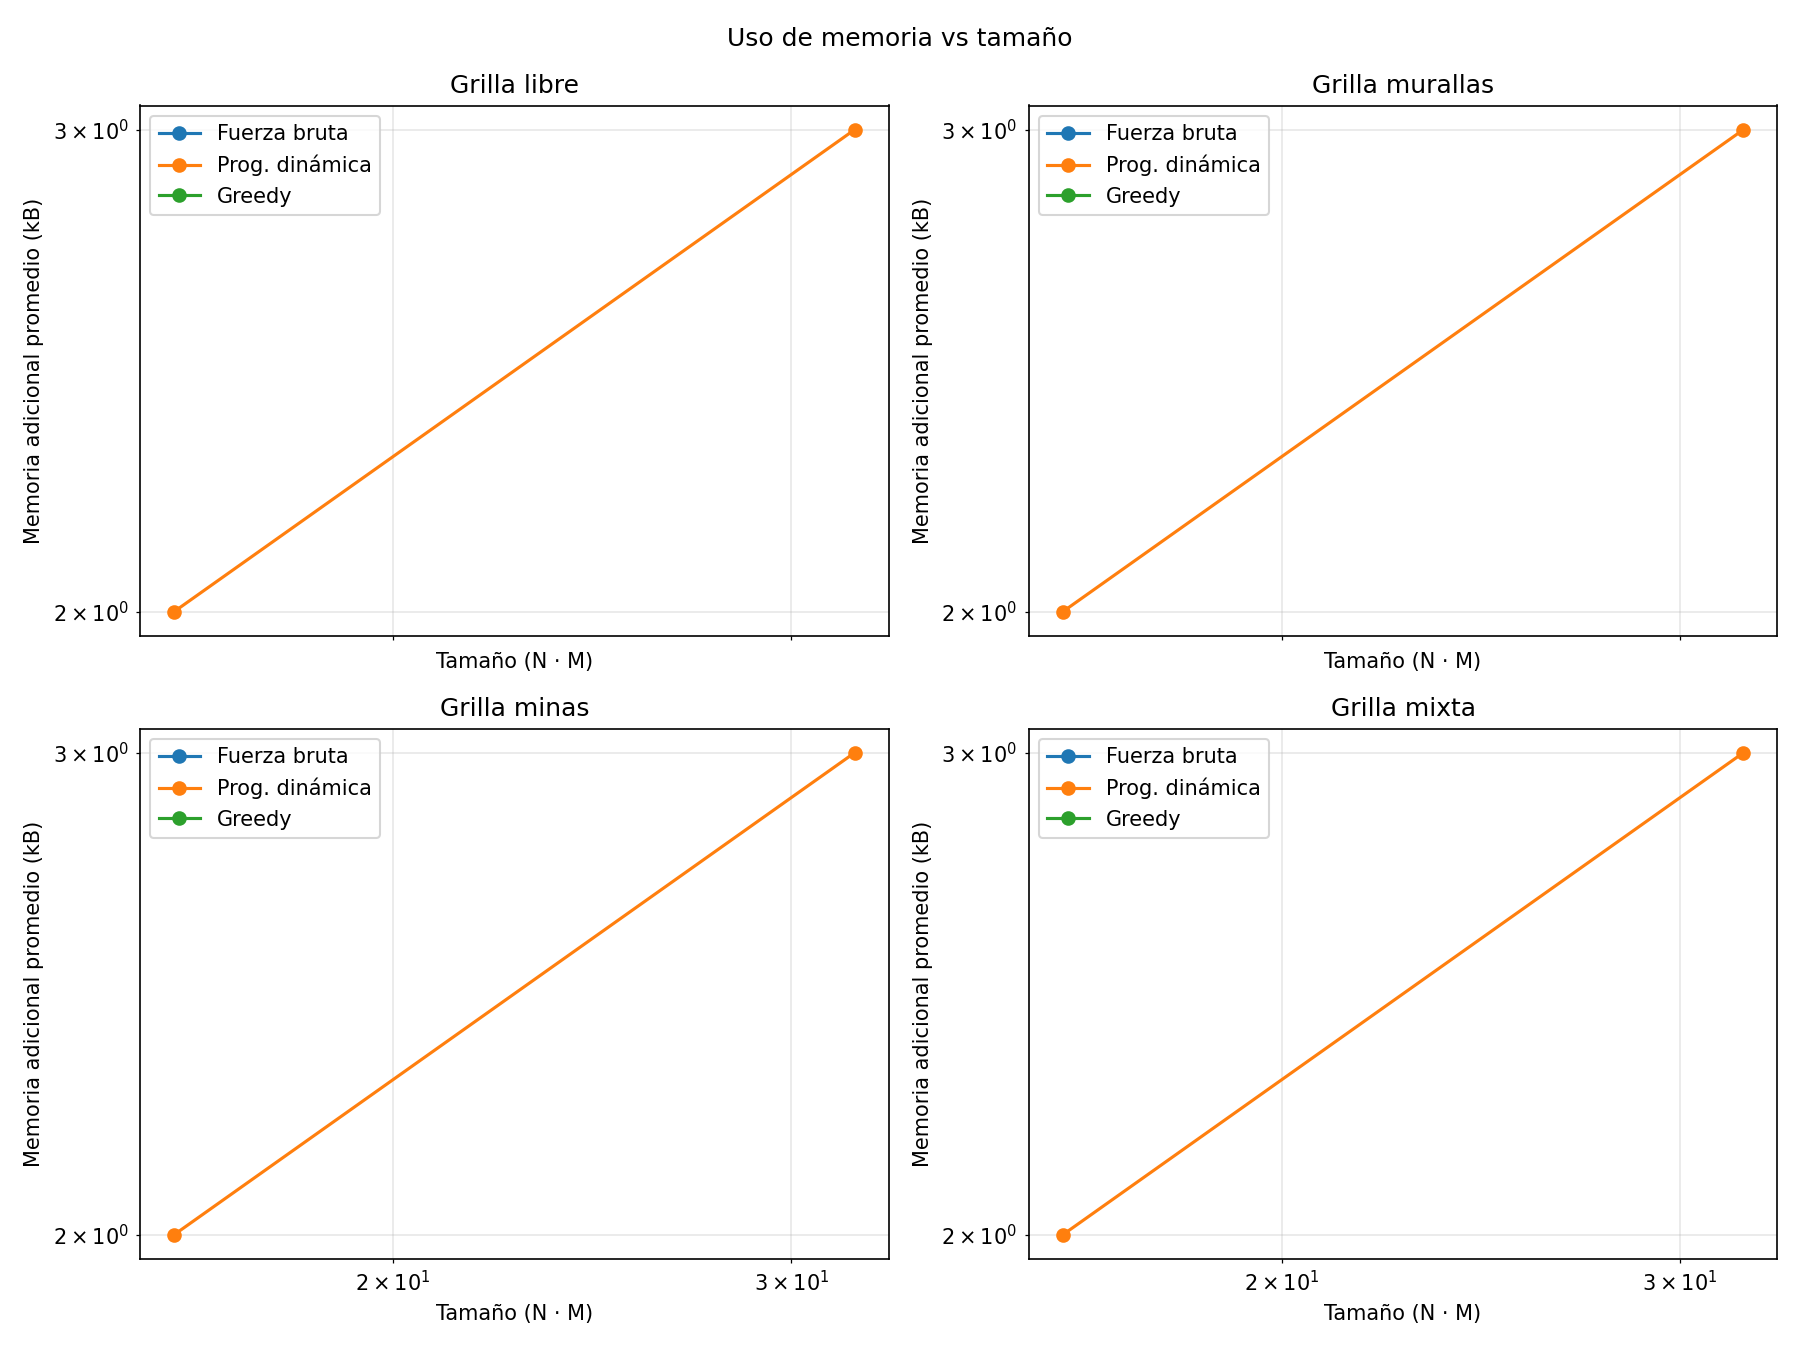
\includegraphics[width=0.8\textwidth]{plots/memoria_vs_tamano.png}
  \caption{Memoria adicional promedio vs tama\~no ($N\cdot M$), por tipo de grilla.}
  \label{fig:memoria}
\end{figure}
 
La memoria medida fue 0~kB para fuerza bruta y greedy, y 2 y 3~kB para DP en
16 y 32 celdas. Teóricamente DP necesita unos $N\cdot M\cdot V\cdot 9$~bytes
(432 y 864~bytes aqu\'i), por lo que el orden de magnitud y el crecimiento son
coherentes, pero la medici\'on por RSS tiene granularidad de p\'aginas del
sistema operativo y a estos tama\~nos no distingue diferencias reales: los
ceros no significan que fuerza bruta y greedy no usen memoria, sino que
est\'an bajo la resoluci\'on del instrumento. Por eso la
Figura~\ref{fig:memoria} solo muestra una curva visible (DP) y no permite
comparar los tres paradigmas de forma concluyente.
 
\subsection{Resumen num\'erico}
La Tabla~\ref{tab:resumen} resume los valores para tama\~nos representativos.
 
\begin{table}[H]
  \centering
  \caption{Tiempo y memoria promedio por tama\~no (promedio sobre tipos, dominios y muestras).}
  \label{tab:resumen}
  \begin{tabular}{rrrrrrr}
    \toprule
    & \multicolumn{3}{c}{Tiempo (ms)} & \multicolumn{3}{c}{Memoria (kB)}\\
    \cmidrule(lr){2-4}\cmidrule(lr){5-7}
    $N\times M$ & BF & DP & Greedy & BF & DP & Greedy\\
    \midrule
    $4\times4$ & 0,0103 & 0,0429 & 0,0017 & 0 & 2 & 0\\
    $4\times8$ & 0,0543 & 0,0544 & 0,0020 & 0 & 3 & 0\\
    \bottomrule
  \end{tabular}
\end{table}
 
\subsection{Calidad de las soluciones de greedy}
La brecha se calcula solo sobre las instancias en que greedy encontr\'o un
camino, tomando como \'optimo el puntaje de DP. Las
Figuras~\ref{fig:brecha_abs} y~\ref{fig:brecha_pct} muestran la brecha absoluta
y relativa seg\'un tama\~no, tipo de grilla y dominio.
 
\begin{figure}[H]
  \centering
  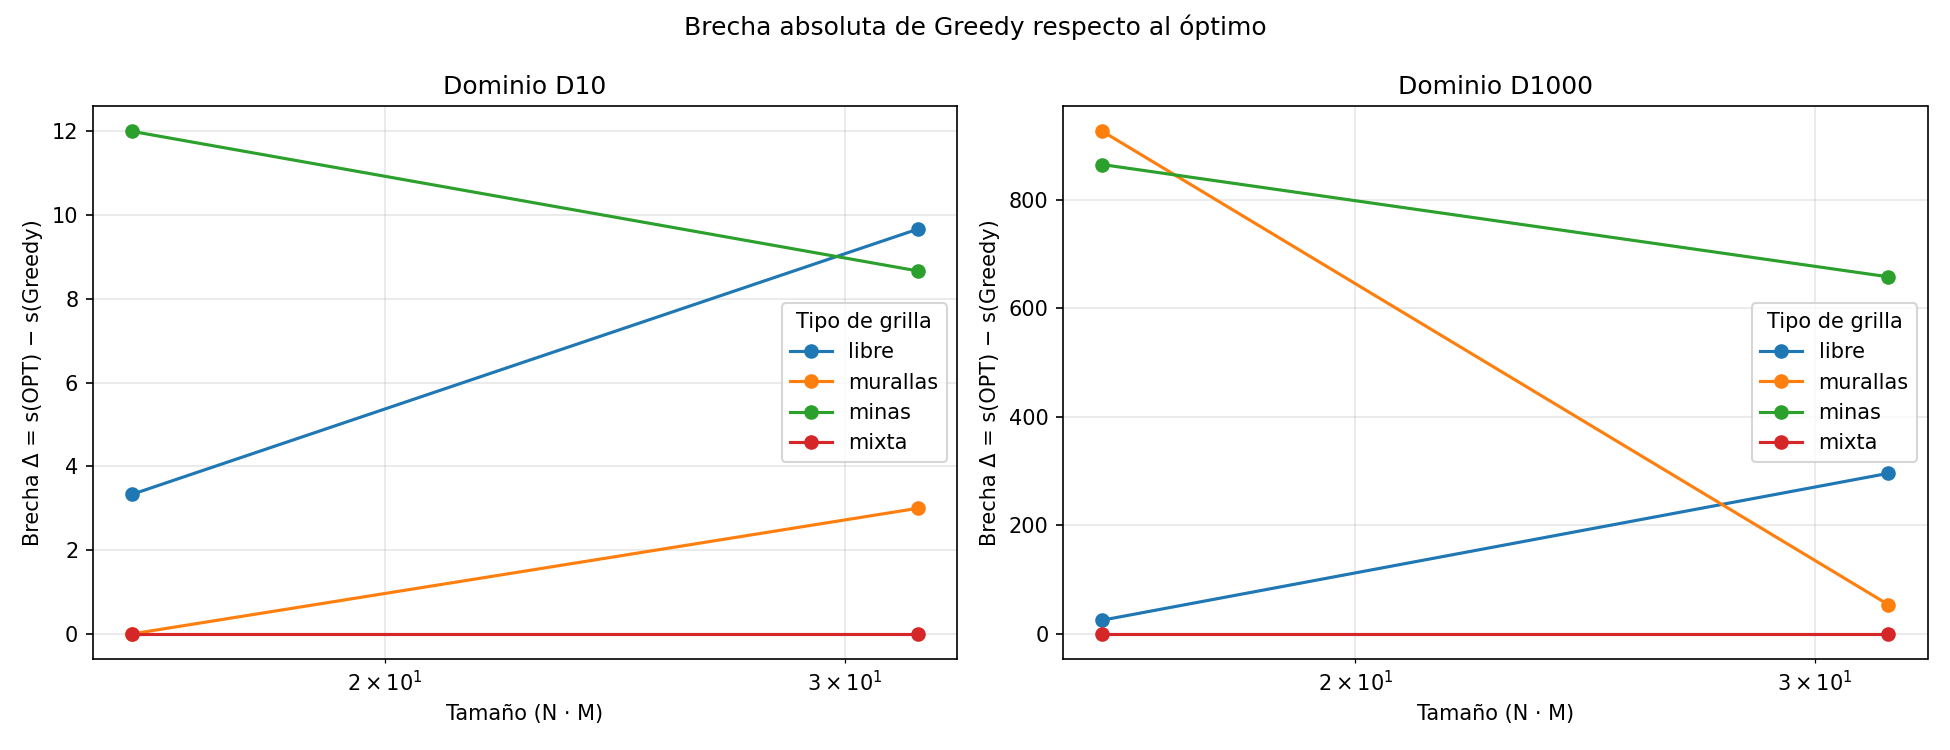
\includegraphics[width=0.8\textwidth]{plots/brecha_abs_greedy.png}
  \caption{Brecha absoluta $\Delta$ de greedy respecto al \'optimo, por dominio y tipo de grilla.}
  \label{fig:brecha_abs}
\end{figure}
 
\begin{figure}[H]
  \centering
  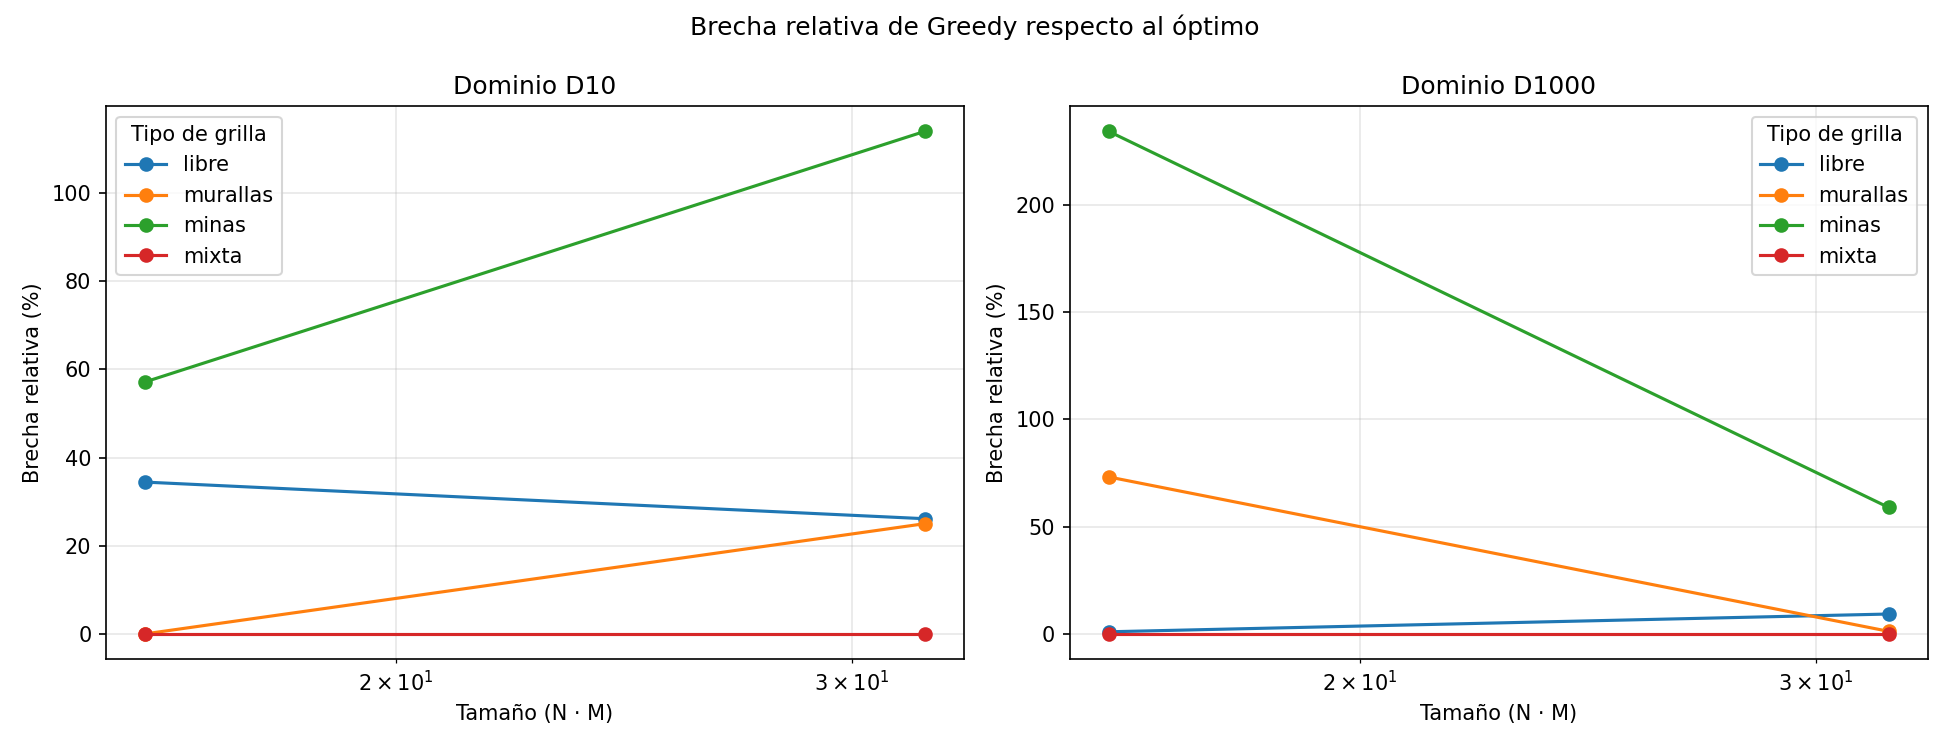
\includegraphics[width=0.8\textwidth]{plots/brecha_pct_greedy.png}
  \caption{Brecha relativa (\%) de greedy respecto al \'optimo, por dominio y tipo de grilla.}
  \label{fig:brecha_pct}
\end{figure}
 
La brecha $\Delta$ nunca fue negativa en las 40 instancias donde greedy
encontr\'o camino, como corresponde a un \'optimo. La brecha promedio fue
217,4 puntos (56,3\,\%) en $4\times4$ y 159,4 puntos (35,7\,\%) en $4\times8$,
es decir, no creci\'o con el tama\~no en este rango; con solo dos tama\~nos
peque\~nos no se puede extrapolar. Por tipo de grilla (brecha relativa
promedio, D10/D1000): libre 30,3\,\%/5,1\,\%, murallas 16,7\,\%/37,2\,\%,
minas 85,6\,\%/146,5\,\%. Las grillas con minas son donde greedy m\'as se aleja
del \'optimo, lo que es esperable: una decisi\'on local no anticipa que sacrificar
una vida puede habilitar mejores sectores. Para la grilla mixta la brecha
promedio fue 0\,\% porque solo se promedian las instancias que greedy resolvi\'o
(4 de 6 en D10 y 5 de 6 en D1000), sin que eso indique mejor calidad.
Los porcentajes deben leerse con cautela: cada celda del an\'alisis reune a lo
m\'as 6 instancias y, cuando el puntaje \'optimo es cercano a cero, la brecha
relativa se infla.
 
La Figura~\ref{fig:falla} y la Tabla~\ref{tab:falla} muestran la tasa de falla
de greedy, es decir, el porcentaje de instancias donde no encontr\'o camino
aunque existe al menos uno v\'alido.
 
\begin{figure}[H]
  \centering
  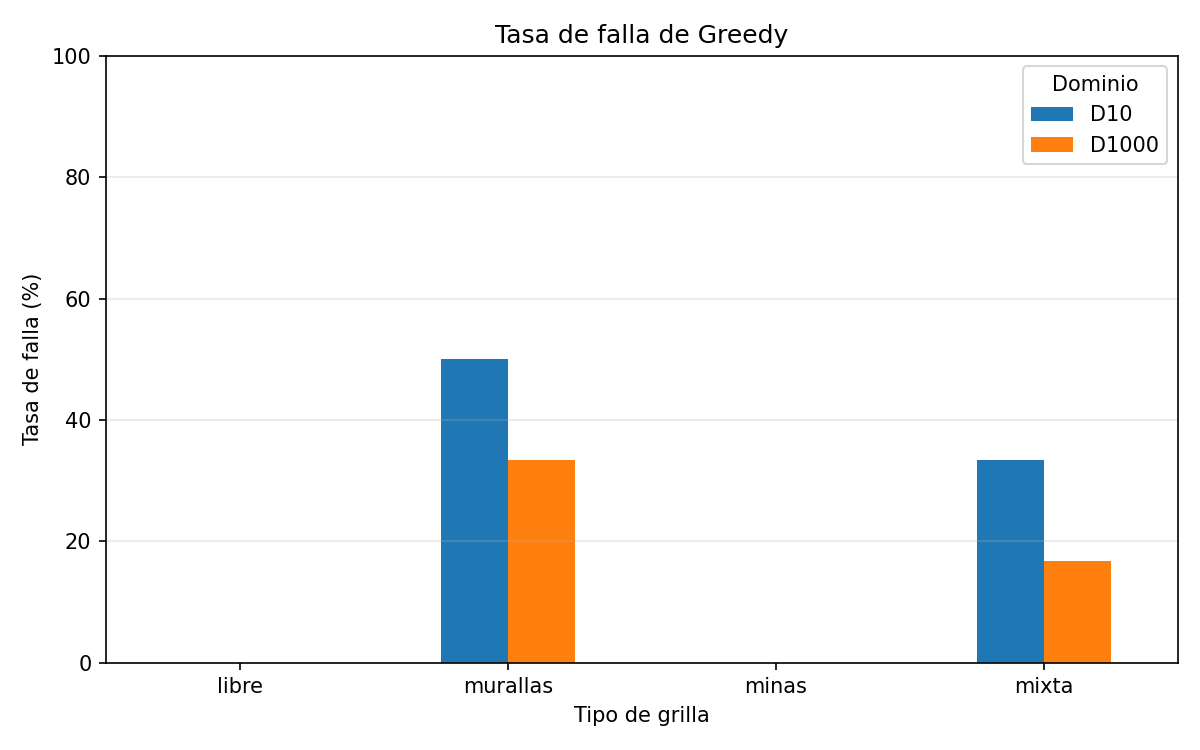
\includegraphics[width=0.7\textwidth]{plots/tasa_falla_greedy.png}
  \caption{Tasa de falla de greedy por tipo de grilla y dominio.}
  \label{fig:falla}
\end{figure}
 
\begin{table}[H]
  \centering
  \caption{Tasa de falla de greedy (\%) por tipo de grilla y dominio.}
  \label{tab:falla}
  \begin{tabular}{lrr}
    \toprule
    Tipo de grilla & D10 & D1000\\
    \midrule
    Libre    & 0,0 & 0,0\\
    Murallas & 50,0 & 33,3\\
    Minas    & 0,0 & 0,0\\
    Mixta    & 33,3 & 16,7\\
    \bottomrule
  \end{tabular}
\end{table}
 
Greedy no fall\'o en grillas libres ni con minas, pues sin murallas siempre
puede avanzar, y solo se bloque\'o en grillas con murallas (50\,\% en D10 y
33,3\,\% en D1000) y mixtas (33,3\,\% y 16,7\,\%). En total fall\'o en 8 de 48
instancias; por tama\~no, 12,5\,\% en $4\times4$ y 20,8\,\% en $4\times8$,
lo que sugiere (sin ser concluyente) que m\'as celdas aumentan la probabilidad
de quedar encerrado. La diferencia entre dominios corresponde a una o dos
instancias por celda, por lo que no se aprecia un efecto claro del dominio.
 